\documentclass[../main.tex]{subfiles}
\graphicspath{{\subfix{../img/}}}
\begin{document}

\newpage
\section{Konzeptfindung}

Das Endziel ist ein möglichst einfaches und zuverlässiges Gesamtkonzept zu finden, welches robust ist und fehlerunanfällig funktioniert. Dies möchten wir erreichen, in dem wir vorgängig alle Lösungsansätze aus der Technologierecherche, die mit grossen Risiken verbunden sind, erkennen und ausscheiden. Mit den verbleibenden Ansätzen wird ein Morphologischer-Kasten erstellt, um das Gesamtkonzept zu entwickeln. Damit mit dem Morphologischen Kasten die optimale Variante gefunden werden kann, wird zu einigen Teilfunktionen des Fahrzeuges eine Nutzwertanalyse erstellt.

\subsection{Vorauswahl}
    \subsubsection{Fortbewegung}
    Das Fahrzeug muss in der Lage sein, sich an Ort und Stelle um die eigene Achse zu wenden. Somit sind die Optionen Knicklenkung, Achsschenkellenkung und Drehschemellenkung nicht geeignet.
    Das Prinzip 'Fahrzeug abbocken und drehen' ist als alleiniges Lenksystem ungeeignet, weil es zu viel Zeit benötigt für das Lenkmanöver. Es wird als optionalen Plan-B beibehalten für den Fall, dass das Fahrzeug beim Wenden während dem Hindernishandling verrutscht. Falls dieses Problem beim Testen auftritt, kann das System nachgerüstet werden.
    Omniwheels und Mecanum-Räder sind sehr ähnlich, nur die Form und Anordnung der Rollen auf den Rädern ist unterschiedlich. Bei Omniwheels sind die Rollen in einem Winkel von 90° an den Rädern befestigt, wobei sie bei Mecanum-Rädern in 45° angeordnet sind und eine Tonnenform aufweisen. Dadurch versprechen die Mecanum-Räder eine geringere Anfälligkeit, sich in den Plattenfugen zu verfangen. Die 4-Rad Differenzial Lenkung und das Prinzip Roomba sind von der Wendigkeit und dem konstruktiven Aufwand vergleichbar, jedoch besteht bei der 4-Rad Variante die Gefahr von Aufschaukeln bei einer Drehung an Ort und Stelle, sowie die Gefahr von Schieben der langsameren Räder bei Kurvenfahrt.
        
    \newpage
    \subsubsection{Hindernis Bewältigung}
        \paragraph{Aufnahme}
        Weil das Konzept möglichst einfach und zuverlässig gestaltet werden soll, scheiden die Ideen 'Gabelstapler' und 'Vakuumgreifer' aus. Der Gabelstapler erfordert eine äusserst präzise und aufwendige Sensorik, um die Löcher für die Aufnahme genau zu treffen. Der Vakuumgreifer dagegen zeigt im Vergleich zu den 'Klemmen' eine geringere Sicherheit in der Technik. Wir besitzen kein Wissen mit dieser Technologie. Um eine vergleichbare Sicherheit zu erreichen, wären umfangreiche Tests erforderlich. Dabei hat der Vakuumgreifer keine signifikanten Vorteile gegenüber den 'Klemmen'. Darum wird der 'Vakuumgreifer' ausgeschlossen.
        
        \paragraph{Rotation und Translation}
        Ein beweglicher Arm erhöht die Komplexität sowohl mechanisch als auch in den Bereichen Sensorik und Software erheblich. Dabei ist zu beachten, dass die Integration eines Arms die Gesamtkomplexität steigert, ohne in anderen Bereichen nennenswerte Vereinfachungen zu ermöglichen, sodass kein Vorteil gewonnen wird. Dies widerspricht unserem Grundprinzip, eine möglichst einfache und zuverlässige Lösung zu entwickeln. Daher werden alle Optionen mit einem beweglichen Arm ausgeschlossen, sodass lediglich die Option "Rotation des Fahrzeugs" verbleibt.


\newpage
\subsubsection{Wegfindung}

Der zu befahrende Graph ist bereits vorgegeben. Er hat acht Knoten und 15 Kanten, was 
für einen Algorithmus relativ klein ist. Die Effizienz und Dynamik des Algorithmus spielt keine grosse Rolle, weil der Zeitunterschied der Algorithmen bei einer Neuberechnung nur minimal ist. Dafür werden Kriterien wie geringer Speicherbedarf und niedrige Komplexität höher gewertet.

\textbf{Ausgeschiedene Algorithmen:}

\begin{itemize}
    \item \textbf{Goal directed shortest path queries using precomputed cluster distances}: Aufgrund der hohen Komplexität und Speicherbedarf wird dieser Algorithmus nicht weiter analysiert.
    \item \textbf{Floyd Warshall}: Der Algorithmus fokussiert sich auf die Berechnung von allen kürzesten Pfaden in einem Graphen. Dies entspricht nicht unserem Anwendungsbereich und wird deshalb nicht weiter analysiert.
\end{itemize}

\subsubsection{Objekterkennung}

Bei der Objekterkennung sind die Schnelligkeit und der Ressourcenbedarf sehr wichtige Kriterien.
Da die Erkennung auf einem Raspberry Pi läuft und so viele Bilder pro Sekunde wie möglich analysieren soll, muss sie möglichst schnell und ressourceneffizient sein. 

R-CNN ist von den vier recherchierten Objekterkennungsmethoden die Langsamste und Ressourcen intensivste, weshalb sie bereits in der Vorauswahl ausscheidet.

\newpage
\subsection{Morphologischer Kasten}

    \imageheight{assets/MorphologischerKasten.pdf}{Morphologischer Kasten}{0.88\textheight}


    \subsubsection{Variantenbeschreibung}
    \paragraph{Lösungsvariante A (grün)}
    Die Fortbewegung und Lenkung wird mit dem Prinzip Roomba realisiert, wobei die beiden angetriebenen Räder mittels je eines DC-Motors getrieben werden. Als Notfall-Lenksystem bleibt die Idee des 'Aufbocken und Drehen'. Die Hindernisse werden von der Seite geklemmt und aufgenommen, der Antrieb dazu wird mit einem Schrittmotor realisiert. Mit dem aufgenommenen Hindernis dreht sich das Fahrzeug um die eigene Achse und setzt dieses wieder ab. Mittels Encoder wird die Position der DC-Motoren überprüft. Die Software läuft auf einem Raspberry Pi und die Hardwaresteuerung auf einem Arduino. Die Hindernisse sollen mit einem Infrarot-Sensor erkannt werden. Um eine Redundanz zu erhalten, wird mittels Ultraschallsensor nachkontrolliert, ob wirklich ein Hindernis im Weg steht. Die Pylonen sollen mit der Kamera, welche auch zur allgemeinen Streckenerkennung verwendet wird, erkannt werden. Mittels Infrarot-Sensor soll auch für die Pylonen ein Backup-Signal generiert werden. Mit einem Liniensensor wird überprüft, ob das Fahrzeug sich auch wirklich entlang eines Klebestreifens bewegt. Dasselbe gilt für die Verifizierung von Wegpunkten, welche primär mit einem Farbsensor erkannt werden. Die Software für die Objekterkennung ist ein YOLO, während die Wegfindung auf Dijkstra läuft. Für die Energieversorgung wird ein Lithium-Polymer-Akku eingesetzt.

    \paragraph{Lösungsvariante B (gelb)}
    Die Fortbewegung und Lenkung wird mit Mecanum-Rädern realisiert, wobei die vier Räder mittels je eines Schrittmotors getrieben werden. Als Notfall-Lenksystem bleibt die Idee des 'Aufbocken und Drehen'. Die Hindernisse werden von vorne und hinten geklemmt und aufgenommen, der Antrieb dazu wird mit einem DC-Motor realisiert. Mit dem aufgenommenen Hindernis dreht sich das Fahrzeug um die eigene Achse und setzt dieses wieder ab. Mittels Hallsensor wird die Position des DC-Motors überprüft. Die Software läuft auf einem Raspberry Pi und die Hardwaresteuerung auf einem TinyK22. Die Hindernisse sollen mit einem Ultraschallsensor erkannt werden. Um eine Redundanz zu erhalten, wird mittels Infrarot-Sensor nachkontrolliert, ob wirklich ein Hindernis im Weg steht. Die Pylonen sollen mit einem Infrarot-Sensor erkannt werden und mittels Ultraschall bestätigt werden. Die Fahrstrecke wird mit einem Liniensensor erkannt und mit der Kamera kontrolliert. Wegpunkte werden ebenfalls mit Liniensensoren gesehen und mit einem Farbsensor bestätigt. Die Software für die Objekterkennung ist ein YOLO, während die Wegfindung auf A* läuft. Für die Energieversorgung wird ein Lithium-Ionen-Akku eingesetzt.

    \paragraph{Entscheid Lösungsvariante}
    Umgesetzt wird die Lösungsvariante A (grün).
    
    \subsubsection{Fortbewegung}

    Damit eine genauere Analyse zwischen Mecanum-Rädern und dem Prinzip Roomba durchgeführt werden kann, wird eine Nutzwertanalyse erstellt. Der Gewinner ist das Prinzip Roomba (ersichtlich in Tabelle \ref{tab:nutzwertanalyse_fortbewegung}).

    \begin{table}[H]
        \textbf{Legende:}
        \hspace{1cm}
        \textbf{GW:} Gewichtung
        \hspace{1cm}
        \textbf{BW:} Bewertung
        \hspace{1cm}
        \textbf{PT:} Punkte
        \vskip 3 mm
        \resizebox{\textwidth}{!}{
        \centering
        \renewcommand{\arraystretch}{1.5}
        \scriptsize
        \begin{tabular}[H]{|p{2cm}|p{3cm}|c|c|c|p{2.5cm}|c|c|p{2.5cm}|}
            \hline
            \multicolumn{3}{|c|}{} & 
            \multicolumn{3}{c|}
            {\textbf{Mecanum-Rad}} & 
            \multicolumn{3}{c|}{\textbf{Prinzip Roomba}}\\ \hline
             \textbf{} & \textbf{Erklärung} & \textbf{GW} & \textbf{BW} & \textbf{PT} & \textbf{Begründung} & \textbf{BW} & \textbf{PT} & \textbf{Begründung} \\ 
            \hline
            Manövrierbarkeit & Wie einfach kann in alle Richtungen manövriert werden & 30 & 9 & 270 & Ist in alle Richtungen beweglich ohne vorgängige Drehung & 6 & 180 & Muss drehen, um in eine andere Richtung zu fahren \\
            \hline
            Resistenz gegen Verfangen in Plattenfugen & Wie anfällig sind die Räder auf Verfangen in den Plattenfugen und damit verbundene Fahrfehler & 35 & 5 & 175 & Kleine Rollen am Radumfang, welche in Fugen passen & 8 & 280 & Nur kleines Stützrad, welches in Fugen passt, Stützrad ist passiv für die Lenkung \\
            \hline
            Komplexität & Wie aufwendig ist die Konstruktion und Programmierung & 20 & 4 & 80 & 4 Motoren ansteuern und hoher Rechenaufwand & 8 & 160 & Nur 2 Motoren nötig \\
            \hline
            Kosten & Wie viel kostet die Vorrichtung & 15 & 4 & 60 & 4 Motoren nötig & 8 & 120 & Nur 2 Motoren nötig \\
            \hline
             Nutzwert & \textbf{Gesamtnutzwert} & 100 & & 585 & & & 740 & \\
            \hline
        \end{tabular}
        \normalsize
        }
        \caption{Nutzwertanalyse Fortbewegung}
        \label{tab:nutzwertanalyse_fortbewegung}
    \end{table}

\subsubsection{Ersatz Rotation}

Das Risiko R15 "Verschieben bei Drehung" (siehe Kapitel \ref{risikomatrix}) wird mitigiert,
in dem optional eine zusätzliche Funktion für das Drehen des Fahrzeugs eingebaut werden kann, falls das Risiko eintreten sollte.

Bei dieser Ersatz-Rotation würde das Fahrzeug aufgebockt werden um sich zu drehen.
Diese Methode ist zwar viel langsamer, würde jedoch sicherstellen, dass sich das Fahrzeug 
beim Drehen nicht verschiebt.

\subsubsection{Fahrantrieb}
Bei der Auslegung des Antriebs ergaben sich drei Varianten. Der Schrittmotor, DC-Motor und der Brushlessmotor. Da die Ansteuerung möglichst einfach gehalten werden soll, ist der Brushlessmotor mit seiner komplexeren Ansteuerung ungeeignet. Der Vorteil des Schrittmotors ist, dass dieser nicht unbedingt auf einen Encoder oder ähnliches angewiesen ist. Dieser kann man genau schrittweise ansteuern und somit seine Position verfolgen. Der Nachteil ist, dass es ein Open-Loop Regelung wäre, also ohne Rückführgrösse. Dies bedeutet bei einer mechanischen Überlastung, würde der Schrittmotor trotz allem die nicht gefahrenen Schritte zurückmelden. Auch dieser Motor hat eine schwierigere Ansteuerung mithilfe von Drivers. Der DC-Motor ist dagegen der einfachste zum Ansteuern. Dieser benötigt eine H-Brücke, die einfach anzusteuern ist. Ausserdem kann man hohe Drehmoment mittels Übersetzungen erreichen. Das macht den DC-Motor zum bevorzugten Antriebsmotor für die Fahrt.


\subsubsection{Hindernisbewältigungsantrieb}
Für die Hindernisbewältigung wird ebenfalls ein Antrieb benötigt. Dafür wird ein Schrittmotor verwendet. Die aufgeführten Nachteile verlieren in der Hindernisbewältigung an Gewichtung. Da ein Motor mit hohem Drehmoment bei niedriger Drehzahl benötigt wird. Somit kann ein Getriebe eingespart werden. Wird das Hindernis geklemmt, ist die minimale Schrittanzahl bekannt. Diese kann überschritten werden. Klemmt der Schrittmotor das Hindernis bereits vor den minimalen Schritten, hat das nicht Erkennen von nicht gemachten Schritten keinen Einfluss. Die Ausgangsposition kann mittels Endschaltern überprüft werden.
  

\subsubsection{Sensorik Positionsabfrage}
Zur Auswahl stehen ein Encoder und ein Hallsensor. Der Encoder liefert genauere Daten und der Aufbau ist einfacher. Daher wird ein Encoder verwendet. Der Encoder kann wichtig sein, um die Fahrtrichtung zu kontrollieren. Sind die verwendeten DC-Motoren nicht identisch, so kann ein anderes Fahrverhalten pro Motor entstehen. Durch einen Encoder kann das Fehlverhalten abgefangen und korrigiert werden.

 Für die korrekte Positionierung der Klemmbacken nach einer Hindernisbewältigung werden Endschalter verwendet. Dadurch wird sichergestellt, dass die Greifarme nach der Hindernisbewältigung wieder in der korrekten Ausgangslage sind.

\subsubsection{Software Steuerung}

Bei der Softwaresteuerung kommt wegen der Grösse und Leistung nur das Raspberry Pi in Frage.
Eine Alternative wäre noch ein Arduino, jedoch reicht dies für leistungsintensive Aufgabe wie
Objekterkennung nicht aus.

\subsubsection{Hardware Steuerung}
Damit man die Aktoren und Sensoren auswerten kann, benötigt es eine Hardware nahe Steuerung, die mit dem Raspberry kommuniziert. Aus der Recherche ergaben sich dafür drei Möglichkeiten. Ein Arduino, TinyK22 oder ein ESP32. Dabei scheidet der ESP32 vor allem durch seine nicht benötigten Funktionen aus. Da es weder Wi-Fi noch Bluetooth benötigt. Damit bleiben noch der TinyK22 und ein Arduino-Board. Aufgrund Ihrer Ähnlichkeit wurde eine Nutzwertanalyse erstellt (siehe Tabelle \ref{tab:konzept_nutzwertanalyse_mikrocontroller}).

    \begin{table}[H]
        \textbf{Legende:}
        \hspace{1cm}
        \textbf{GW:} Gewichtung
        \hspace{1cm}
        \textbf{BW:} Bewertung
        \hspace{1cm}
        \textbf{PT:} Punkte
        \vskip 3 mm
        \resizebox{\textwidth}{!}{
         \centering
         \renewcommand{\arraystretch}{1.5}
             \begin{tabular}{|p{2.5cm}|>{\raggedright} p{3cm}|c|c|c|>{\raggedright} p{3cm}|c|c|>{\raggedright\arraybackslash}p{3cm}|}
                \hline
                \multicolumn{3}{|c|}{} & \multicolumn{3}{c|}{\textbf{Arduino}} & \multicolumn{3}{c|}{\textbf{TinyK22}} \\ \hline
                \textbf{Kriterium} & \textbf{Erklärung} & \textbf{GW} & 
                \textbf{BW} & \textbf{PT} & 
                \textbf{Begründung} & \textbf{BW} & 
                \textbf{PT} & \textbf{Begründung} \\ \hline

                Libraries & Sind Frameworks vorhanden & 20 & 9 & 180 & Grosse Anzahl Online Libraries & 8 & 160 & McFun Bibliothek \\ \hline
                Online Informationen & verfügbare Skripte / Beschriebe vorhanden? & 30 & 8 & 240 & Viele Online Tutorials & 6 & 180 & Blog von M. Styger und McFun Folien \\ \hline
                I/O Pins & Anzahl frei verfügbare GPIO & 30 & 6 & 180 & 22 Pins beim nano & 8 & 240 & 28 Pins verfügbar \\ \hline
                Finanziell & Wie viel kostet der Mikrocontroller & 10 & 6 & 60 & Um die 20CHF & 9 & 90 & Evtl. von der Schule \\ \hline
                Nachhaltigkeit & Energieverbrauch für die Beschaffung & 10 & 7 & 70 & Arduino bereits von Privatgebrauch vorhanden & 9 & 90 & Bereits vorhanden aus früheren Modulen \\ \hline
                \multicolumn{2}{|r|}{\textbf{Nutzwert:}} & 100 & & 730 & & & 760 & \\ \hline
            \end{tabular}
         }
            \caption{Nutzwertanalyse der Mikrocontroller}
            \label{tab:konzept_nutzwertanalyse_mikrocontroller}
        \end{table}

    Da der Unterschied nicht sehr gross ist, wird als erste Wahl der Arduino verwendet und das TinyK22 als Ersatzwahl. Allenfalls könnten beide Boards verwendet werden und die dann miteinander kommunizieren. Beispielsweise gibt es ein Arduino mit zwei UART Schnittstellen. Dieses kann als Kommunikator zum Raspberry und TinyK22 dienen. Hintergrund ist, dass eine Software für die Motorensteuerung per TinyK22 bereit besteht, mit welcher Thomas und Joel bereits gearbeitet haben. Ausserdem würden mit dieser Lösung mehr GPIOs bereitstehen, damit man im Projekt agil reagieren kann und keine Hardwaremässigen Limits hat.

\subsubsection{Objekterkennung Hardware}
 Bei der Wahl der richtigen Sensorik müssen noch Tests durchgeführt werden. Damit bewertet werden kann, welcher Sensor sich bei der vorgegebenen Umwelt am besten verhält. Vor allem für den Liniensensor und für die Erkennung des Wegpunktes. Da der Untergrund keine kontrastreichen Flächen hat. Für die Distanzmesssensoren ist ein Test zum Vergleich der Präzision zwischen Ultraschall und IR ebenso notwendig.
 
 Bereits angedacht ist, dass  die wichtigsten Sensoren doppelt abgedeckt werden sollen (siehe Risikoanalyse). So ist eine weitere Möglichkeit vorhanden, falls ein Sensor nicht die gewünschten Daten liefert. Als Beispiel werden Farbsensoren gegen den Boden gerichtet sein, wie auch Fototransistoren mit LEDs, um die weissen Wegpunkte zu erkennen.

\subsubsection{Streckenerkennung}
Für die Streckenerkennung soll eine Kamera verwendet werden. Ein zweiter Lösungsansatz ist der Linienfolger. Um die Funktionalität eines Linienfolger zu verifizieren, muss dieser in der Fahrumgebung getestet werden. Ebenfalls muss getestet werden, wie gut die Kamera die Linien bei starker Reflexion erkennt. Mit den Messresultaten wird entschieden, welche Methode umgesetzt wird.


\subsubsection{Punktverifizierung}
Um zu erkennen, ob das Fahrzeug sich auf ein Punkt befindet, wird ein Farbsensor genutzt. Dieser gibt die drei Primärfarben in je einem Digitalsignal zurück. Ausserdem wird die Farbtemperatur in Kelvin zurückgegeben. Mit diesen Werten kann man das leicht gelbe Klebeband von dem weissen Punkt unterscheiden. Dies ermöglicht es am einfachsten den weissen Punkt zuerkennen. Eine weitere Option wäre die Erkennung mittels eines kreisförmigen Liniensensors. Mit diesem kann man die Form der Linie erkennen. Wenn das Fahrzeug auf dem Punkt steht, haben alle Phototransistoren den gleichen Wert. Diese Variante ist ein empfindlicher und es setzt voraus, dass das Fahrzeug zentriert auf der Linie fährt. Die Variante mit der Kamera scheidet aus, da es zu teuer wäre zwei Kameras zu nutzen. Weil damit je nach Kamera 1/5 des Budgets aufgebraucht wäre. Es würden zwei benötigt, da die eine Kamera, die für die Strecken und Objekterkennung ist, sich auf einer gewissen Höhe befinden muss. Dagegen muss die Linienkamera möglichst nah an der Linie sein.


\subsubsection{Objekterkennung Software}


Bei der Technologierecherche wurden vier verschiedene Objekterkennungsmethoden recherchiert, wobei eine davon bei der Vorauswahl ausschied. 
Dieser Abschnitt fokussiert sich darauf, anhand von einer Nutzwertanalyse von den restlichen drei Auswahlen die Beste zu treffen.

Für die Nutzwertanalyse werden die folgenden Kriterien verwendet.

\begin{itemize}
\item \textbf{Genauigkeit}: Das wichtigste Kriterium ist, dass alle Objekte, die in einem Bild ersichtlich sind, genau erkannt werden.
\item \textbf{Geschwindigkeit}: Die Bilder werden während des Fahrens analysiert. Eine schnelle Objekterkennungsmethode ist essenziell, damit das Fahrzeug schnell reagieren kann.
\item \textbf{Ressourcenbedarf}: Die Objekterkennung erfolgt on-board auf ressourcenlimitierter Hardware. Somit soll die Erkennung möglichst effizient sein.
\item \textbf{Komplexität}: Das Projekt ist zeitlich limitiert. Der Aufwand für die Implementierung der Objekterkennung berücksichtigt werden. Dazu gehört auch die Menge der benötigten Trainingsdaten.
\end{itemize}

\begin{table}[H]
\resizebox{\textwidth}{!}{
 \centering
 \renewcommand{\arraystretch}{1.5}
     \begin{tabular}{|c|c|c|c|c|c|c|c|}
        \hline
        \multicolumn{2}{|c|}{} & 
        \multicolumn{2}{c|}{\textbf{CNN}} &
        \multicolumn{2}{c|}{\textbf{YOLO}} &
        \multicolumn{2}{c|}{\textbf{Haar-Cascade}} \\
        \hline
        
        \textbf{Kriterium} & \textbf{Gewicht} &
        \textbf{Bewertung} & \textbf{Punkte} &
        \textbf{Bewertung} & \textbf{Punkte} &
        \textbf{Bewertung} & \textbf{Punkte} \\
        \hline

        Genauigkeit & 40 &
        8 & 320 &
        7 & 280 &
        5 & 200 \\
        \hline

        Geschwindigkeit & 30 &
        6 & 180 &
        9 & 270 &
        8 & 240 \\
        \hline

        Ressourcenbedarf & 20 &
        4 & 80 &
        6 & 120 &
        8 & 160 \\
        \hline

        Komplexität & 10 &
        2 & 20 &
        5 & 50 &
        7 & 70 \\
        \hline
        
        \textbf{Nutzwert:} & 100 & & 590 & & 720 & & 670 \\ \hline
    \end{tabular}
 }
    \caption{Nutzwertanalyse Objekterkennung}
    \label{tab:nutzwertanalyse_objekterkennung}
\end{table}

YOLO erreicht in der durchgeführten Nutzwertanalyse (siehe Tabelle \ref{tab:nutzwertanalyse_objekterkennung}) die beste Gesamtbewertung. Es erlaubt eine effiziente und relativ genaue Analyse der Bilder.
Haar-Cascade ist ebenfalls schnell und ressourcenschonend, schneidet aber in der wichtigsten Kategorie ''Genauigkeit'' schlecht ab.
CNN, das in der Kategorie Genauigkeit die beste Bewertung erzielte, zeigt deutliche Schwächen in Bezug auf ''Geschwindigkeit'', ''Ressourcenbedarf'' und ''Komplexität''.

\subsubsection{Wegfindung}

Der geeignetste Wegfindungsalgorithmus wird anhand einer Nutzwertanalyse mit den folgenden Kriterien gefunden.

\begin{itemize}
    \item \textbf{Einfachheit:} Einfach zu implementieren oder bereits in bekannten Bibliotheken vorhanden.
    \item \textbf{Genauigkeit:} Findet \textbf{garantiert} den kürzesten Weg.
    \item \textbf{Dynamisch:} Kann sich dynamisch auf Graphveränderungen anpassen.
    \item \textbf{Schnelligkeit:} Wie schnell der kürzeste Weg berechnet werden kann.
    \item \textbf{Effizienz:} Benötigter Leistungs- und Speicheraufwand
\end{itemize}

\begin{table}[H]
\resizebox{\textwidth}{!}{
 \centering
 \renewcommand{\arraystretch}{1.5}
     \begin{tabular}{|c|c|c|c|c|c|c|c|c|c|}
        \hline
        \multicolumn{2}{|c|}{} & 
        \multicolumn{2}{c|}{\textbf{Dijkstra}} &
        \multicolumn{2}{c|}{\textbf{A*}} &
        \multicolumn{2}{c|}{\textbf{D*}} &
        \multicolumn{2}{c|}{\textbf{RRT}} \\ 
        \hline
        
        \textbf{Kriterium} & \textbf{Gewicht} &
        \textbf{Bewertung} & \textbf{Punkte} &
        \textbf{Bewertung} & \textbf{Punkte} &
        \textbf{Bewertung} & \textbf{Punkte} &
        \textbf{Bewertung} & \textbf{Punkte} \\
        \hline

        Einfachheit & 10 &
        10 & 100 &
        7 & 70 &
        5 & 50 &
        3 & 30 \\
        \hline

        Genauigkeit & 60 &
        10 & 600 &
        8 & 480 &
        8 & 480 &
        6 & 360 \\
        \hline

        Dynamisch & 5 &
        1 & 5 &
        1 & 5 &
        10 & 50 &
        5 & 25 \\
        \hline

        Schnelligkeit & 5 &
        7 & 35 &
        8 & 40 &
        9 & 45 &
        5 & 25 \\
        \hline

        Effizienz & 20 &
        9 & 180 &
        7 & 140 &
        4 & 80 &
        2 & 40 \\
        \hline
        
        \textbf{Nutzwert:} & 100 & & 920 & & 735 & & 705 && 480 \\ \hline
    \end{tabular}
 }
    \caption{Nutzwertanalyse Wegfindung}
    \label{tab:nutzwertanalyse_wegfindung}
\end{table}

Die Nutzwertanalyse zeigt Dijkstra als deutlichen Gewinner. Dies liegt vor allem an der hohen Genauigkeit, Einfachheit und Effizient. Einzig bei der nicht vorhandenen Dynamik schneidet Dijkstra schlecht ab. Aufgrund des kleinen Graphen spielt das jedoch keine grosse Rolle, da der Weg einfach neu berechnet werden kann.

\subsubsection{Energiequelle}
Zur Auswahl steht ein Li-Po, Li-Ion oder NiMh Akku. Der Li-Po und Li-Ion Akku haben die höhere Energiedichte als der NiMh Akku. Jedoch benötigt der Li-Po einen Laderegler für die Aufladung und der Li-Ionen benötigt eine elektrische Schutzschaltung. Zwischen dem Li-Ion und dem Li-Po Akku gibt es keine weiteren nennenswerten Unterschiede. 
Im Vergleich zu dem NiMh Akku benötigen sie weniger Platz und sind leichter. Ebenso haben sie keinen Memoryeffekt und eine geringere Selbstentladung als der NiMh Akku. Die Lebensdauer eines NiMh Akkus ist dagegen fast fünfmal so lange wie die eines Lipo-Akkus\footnote{https://www.rcteam.com/de/blogs/der-blog-des-rc-modellbaus/nimh-vs-lipo-batterien}.


\begin{table}[H]
        \resizebox{\textwidth}{!}{
         \centering
         \renewcommand{\arraystretch}{1.5}
             \begin{tabular}{|c|>{\raggedright} p{3cm}|c|c|c|>{\raggedright} p{3cm}|c|c|>{\raggedright\arraybackslash}p{3cm}|}
                \hline
                \multicolumn{3}{|c|}{} & \multicolumn{3}{c|}{\textbf{LiPo}} & \multicolumn{3}{c|}{\textbf{NiMh}} \\ \hline
                \textbf{Kriterium} & \textbf{Erklärung} & \textbf{Gewichtung} & \textbf{Bewertung} & \textbf{Punkte} & \textbf{Begründung} & \textbf{Bewertung} & \textbf{Punkte} & \textbf{Begründung} \\ \hline
                Lebensdauer & Wie lange hält der Akku & 10 & 6 & 60 & Bis 200 Ladezyklen & 8 & 80 & Bis 1000 Ladezyklen \\ \hline
                Leistungsdichte & Energie / Volumen & 30 & 9 & 270 & Hohe Energiedichte & 6 & 180 & Mittlere Energiedichte \\ \hline
                Leistungsabgabe & Wie viel Strom kann gezogen werden & 30 & 8 & 240 & Hohe Entladungsrate  & 4 & 120 & Niedrige Entladungsrate \\ \hline
                Sicherheit & Brenngefahr & 20 & 4 & 80 & Gefahr bei unsachmässigem Gebrauch & 8 & 160 & Keine Gefahr \\ \hline
                Kosten & Wie viel kostet der Akku & 10 & 4 & 40 & Um die 30CHF & 7 & 70 & Um die 20CHF \\ \hline
                \multicolumn{2}{|r|}{\textbf{Nutzwert:}} & 100 & & 690 & & & 610 & \\ \hline
            \end{tabular}
}
            \caption{Nutzwertanalyse Akku}
            \label{tab:konzept_Akku}
        \end{table}
        

Es wird der Li-Po Akku verwendet. Diese Akkus werden hauptsächlich für den Modellbau verwendet. Wie gemacht für einen Prototyp. Der NiMh Akku wird nicht verwendet, da dieser eine geringe Leistungsabgabe hat (siehe auch Tabelle \ref{tab:konzept_Akku})\footnote{https://www.rccrush.com/nimh-vs-lipo-batteries/}. Durch die Bildverarbeitung wird ein leistungsstarker Akku benötigt. Der Entscheid ist aufgrund des vorgesehenen Anwendungsbereiches gegen den Li-Ion Akku gefallen. Durch den Modellbauanwendungsbereich des Li-Po Akkus ist es einfacher ähnliche Anwendungen zu finden.


\newpage
\subsubsection{Aufnahme Hindernis}
\subparagraph{Nutzwertanalyse Aufnahme}
        Damit eine genauere Analyse zwischen Klemme Breitenweg und Klemmung seitlich durchgeführt werden konnte, wurde eine Nutzwertanalyse durchgeführt. Der Gewinner war dank der höheren Präzision Klemme Breitenweg, was auch in Tabelle \ref{tab:konzept_nutzwertanalyse_aufnahme} ersichtlich ist.
        
        \begin{table}[H]
        \resizebox{\textwidth}{!}{
         \centering
         \renewcommand{\arraystretch}{1.5}
             \begin{tabular}{|c|>{\raggedright} p{3cm}|c|c|c|>{\raggedright} p{3cm}|c|c|>{\raggedright\arraybackslash}p{3cm}|}
                \hline
                \multicolumn{3}{|c|}{} & \multicolumn{3}{c|}{\textbf{Klemme Breitenweg}} & \multicolumn{3}{c|}{\textbf{Klemme seitlich}} \\ \hline
                \textbf{Kriterium} & \textbf{Erklärung} & \textbf{Gewichtung} & \textbf{Bewertung} & \textbf{Punkte} & \textbf{Begründung} & \textbf{Bewertung} & \textbf{Punkte} & \textbf{Begründung} \\ \hline
                Sicherer Halt & Wie gut hält das Hindernis in der Halterung & 35 & 7 & 245 & Relativ starke Punktlast, aber dennoch sehr guter Halt & 8 & 280 & Große Fläche zur Kraftübertragung, stabil und sehr guter Halt \\ \hline
                Präzision & Wie präzise ist die Vorrichtung, auch wenn das Fahrzeug nicht genau zentriert vor dem Hindernis steht & 30 & 7 & 210 & Siehe Kapitel Präzision, detaillierte Erklärung & 4 & 120 & Siehe Kapitel Präzision, detaillierte Erklärung \\ \hline
                Komplexität & Wie aufwendig ist die Konstruktion & 20 & 5 & 100 & Nicht sehr komplex & 5 & 100 & Nicht sehr komplex \\ \hline
                Kosten & Wie viel kostet die Vorrichtung & 15 & 4 & 60 & 3D-Druck möglich & 4 & 60 & 3D-Druck möglich \\ \hline
                \multicolumn{2}{|r|}{\textbf{Nutzwert:}} & 100 & & 615 & & & 560 & \\ \hline
            \end{tabular}
         }
            \caption{Nutzwertanalyse Hindernis Aufnahme}
            \label{tab:konzept_nutzwertanalyse_aufnahme}
        \end{table}

        \newpage
            
            \subparagraph{Präzision}

            In der Nutzwertanalyse wird erwähnt, dass das Kriterium Präzision eine präzisere Erklärung benötigt. Die Präzision der Klemme Breitenweg kann besser erreicht werden als bei der Klemmung seitlich. Einerseits kann, wie in den Abbildungen \ref{img:konzept_zentrierung_1} und \ref{img:konzept_zentrierung_2} gezeigt, eine Zentrierung bei der Klemme Breitenweg eingebaut werden. Diese Zentrierung fehlt bei der Klemmung seitlich. Da unter anderem das Ziel ist, das Hindernis möglichst zentriert wieder auf dem Klebeband abzustellen, verliert hier die Klemmung seitlch an Punkten. In Abbildung \ref{img:konzept_zentrierung_3} wird dargestellt, dass, wenn das Fahrzeug nicht perfekt mittig auf das Hindernis zufährt, automatisch ein Fehler generiert wird, weil das 'Offset' nicht, ohne komplexere Sensorik, miteinbezogen werden kann.


            \begin{figure}[h!]
                \centering
                \begin{minipage}{0.48\textwidth}
                    \centering
                    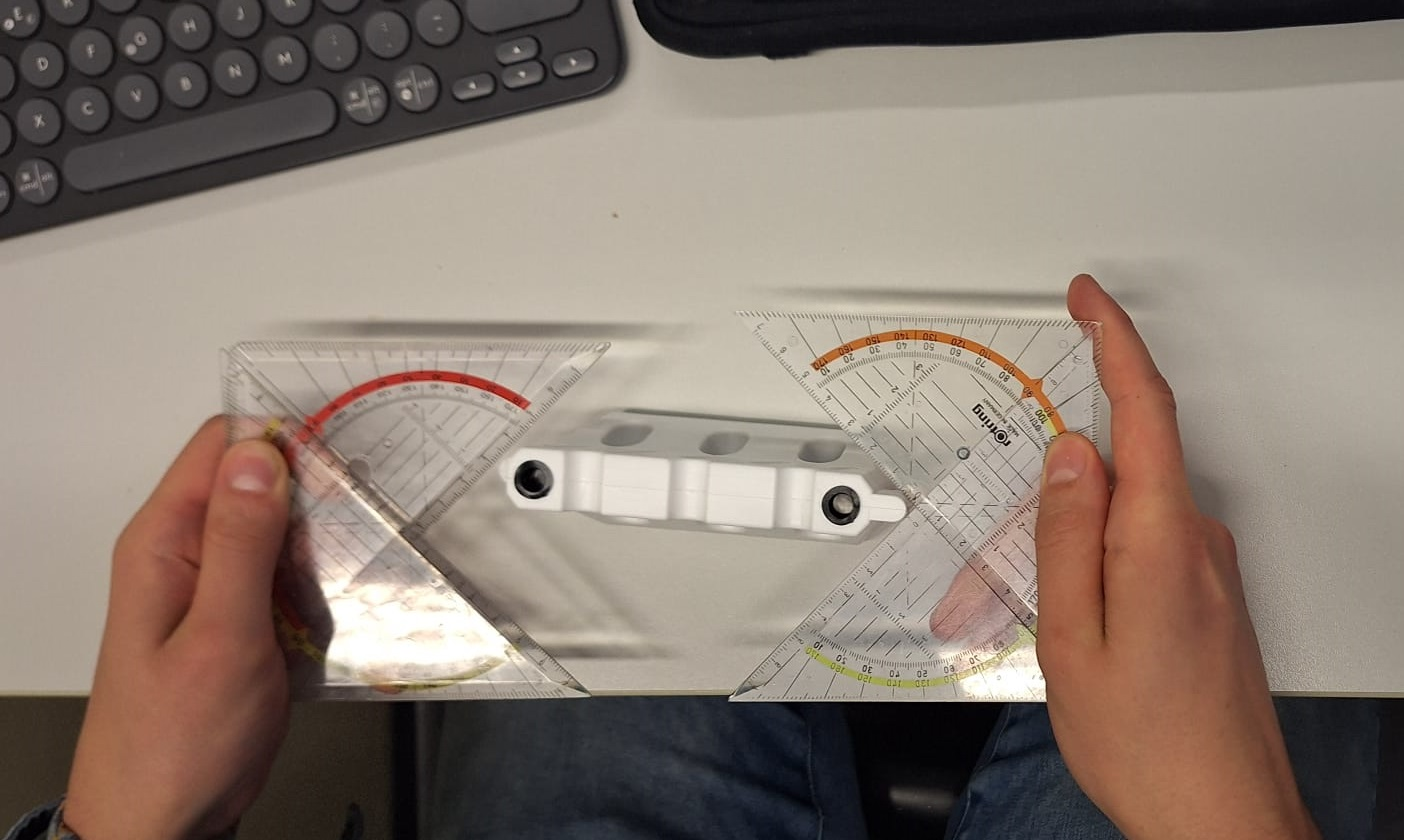
\includegraphics[width=\linewidth]{img/konzeptfindung/klemme_breitenweg_zentrierung_1.jpeg}
                    \caption{Darstellung Zentrierung bei Klemme Breitenweg - Bild 1}
                    \label{img:konzept_zentrierung_1}
                \end{minipage}
                \hfill
                \begin{minipage}{0.48\textwidth}
                    \centering
                    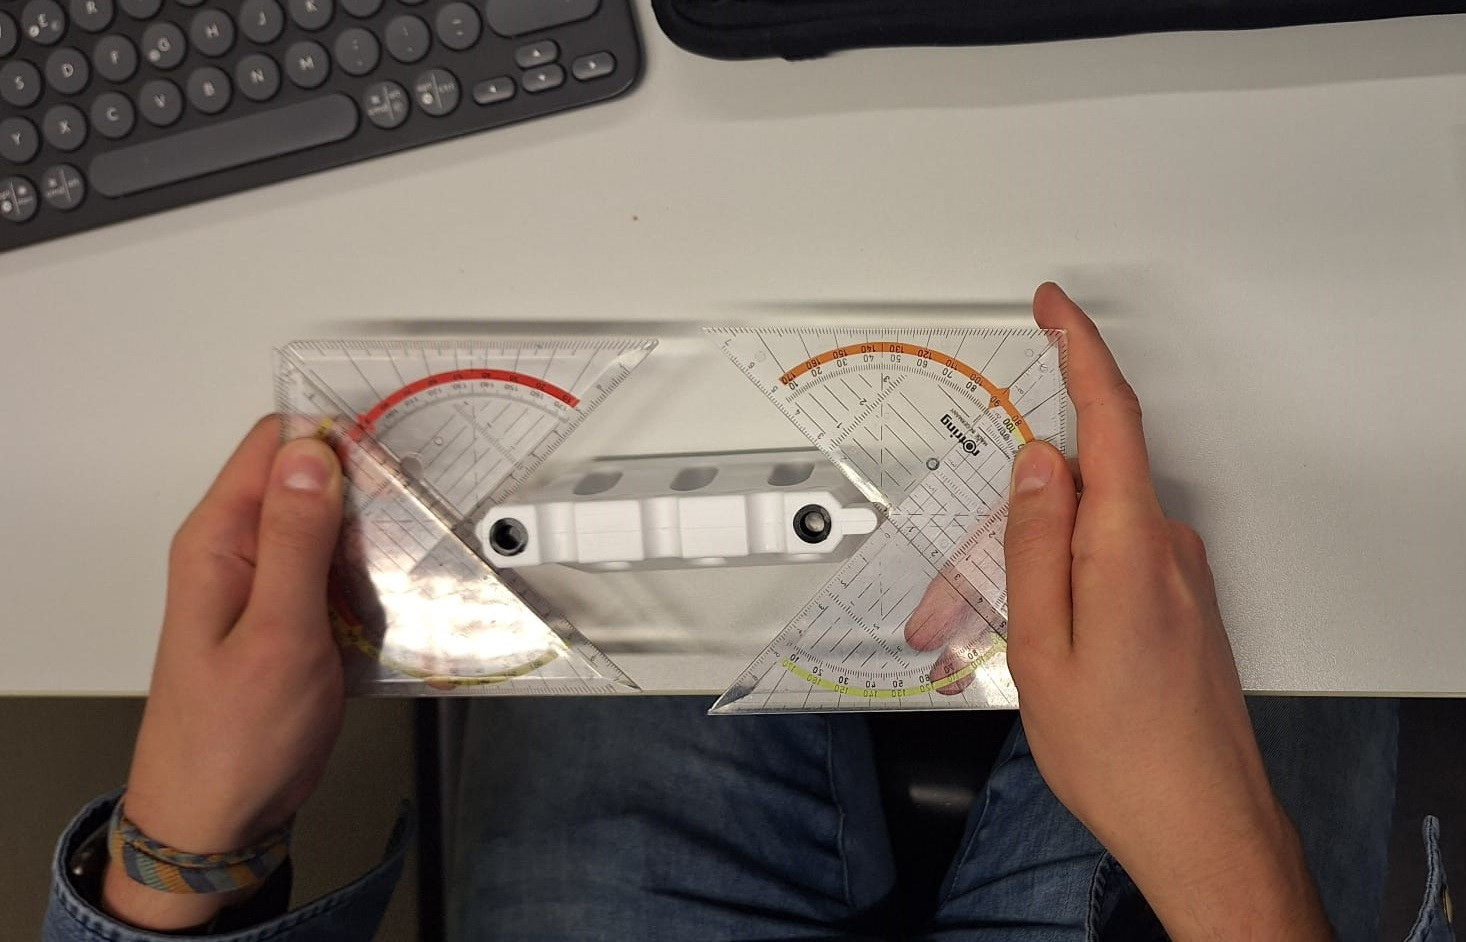
\includegraphics[width=\linewidth]{img/konzeptfindung/klemme_breitenweg_zentrierung_2.jpeg}
                    \caption{Darstellung Zentrierung bei Klemme Breitenweg - Bild 2}
                    \label{img:konzept_zentrierung_2}
                \end{minipage}
            \end{figure}


        \begin{figure}[h!]
            \centering
            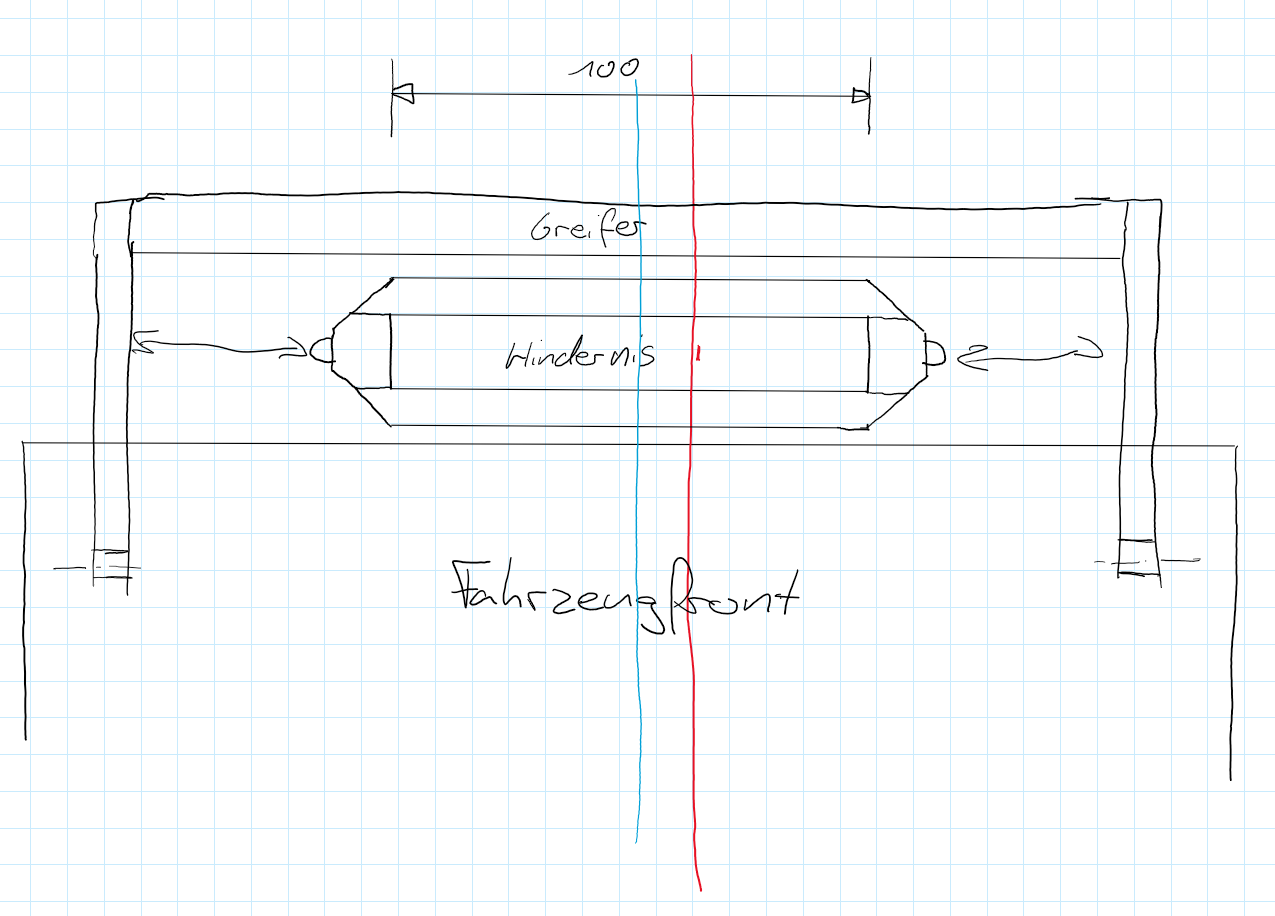
\includegraphics[width=0.48\textwidth]{img/konzeptfindung/Klemme_Langsweg_off_center.png}
            \caption{Darstellung 'Offset' bei Klemmung seitlich}
        \label{img:konzept_zentrierung_3}
        \end{figure}  


\end{document}